\lab{Python}{NumPy Arrays and NumPy and SciPy}{NumPy Arrays and NumPy and SciPy} 
\objective{Create and manipulate powerful NumPy $n$-dimensional arrays and learn features available in NumPy and SciPy.}
\label{lab:NumPyArrays}

\section*{Introduction}

NumPy and SciPy\footnote{SciPy is also the name of a Python coding environment that includes the NumPy and SciPy libraries, as well as IPython, matplotlib, and other tools.} are the two Python libraries most used for scientific computing. NumPy is a package for manipulating vectors and arrays, and SciPy is a higher-level library built on NumPy. The basic object in NumPy is the \emph{array}, which is conceptually similar to a matrix. However, unlike a matrix, which has two dimensions, a NumPy \li{array} can have arbitrarily many dimensions. NumPy is optimized for fast array computations, and you will see in a later exercise [TODO: ref] just what a difference this can make.

The convention is to import NumPy as follows.

\begin{lstlisting}
>>> import numpy as np
\end{lstlisting}

\section*{Learning NumPy}
The strategies discussed in the section ``Learning Python'' of Lab [TODO ref 1] will also help you learn NumPy and SciPy. The following online resources are specific to SciPy.
\begin{itemize}
\item Official SciPy Documentation (\url{http://docs.scipy.org/doc/})
\item Sections 1.3 and 1.5 of the SciPy Lecture Notes (\url{http://scipy-lectures.github.io/})
\end{itemize}
The remainder of this lab is a \emph{brief} summary of the tools available in NumPy and SciPy, beginning with NumPy arrays.


%%%%%%%%%%%%%%%%%%%%%%%%%%%%%%%%%%%%%%%%%%%%%%%%%%%%%%%%%%%
%%%%%%%%%%%%%%%%%%%%%%%%%%%%%%%%%%%%%%%%%%%%%%%%%%%%%%%%%%%
%%%%%%%%%%%%%%%%%%%%%%%%%%%%%%%%%%%%%%%%%%%%%%%%%%%%%%%%%%%
%%%%%%%%%%%%%%%%%%%%%%%%%%%%%%%%%%%%%%%%%%%%%%%%%%%%%%%%%%%
\section*{Arrays}

Conceptually, a 1-dimensional array (called a 1-D array) is just a list of numbers. An $n$-dimensional array (or $n$-D array) is an array of $n-1$-dimensional arrays. Thus, any 2-D array is conceptually a matrix, and a 3-D array is a list of matrices, which can be visualized as a cube of numbers. Each dimension is called an \emph{axis}. When a 2-D array is printed to the screen, the 0-axis indexes the rows and the 1-axis indexes the columns.

The NumPy array class is called \li{ndarray}. The simplest way to create an \li{ndarray} is
to define it explicitly using nested lists.
\begin{lstlisting}
# Create a 1-D array
>>> np.array([0, 3, 8, 6, 3.14])
array([0, 3, 8, 6, 3.14]) 

# Create a 2-D array
>>> b = np.array([[1, 1, 2], [3, 3, 4]]); b
array([[1, 1, 2],
       [3, 3, 4]])
\end{lstlisting} 

You can access the dimension of any array with the command \li{ndim}.
\begin{lstlisting}
>>> b.ndim
2
\end{lstlisting}

You can view the length of each dimension with the \li{shape} command, and change the shape of an array with the \li{np.reshape()} function. The number of arguments passed to \li{reshape} tells NumPy the dimension of the new array, and the arguments specify the length of each dimension. An argument of \li{-1} tells NumPy to make that dimension as long a necessary.
\begin{lstlisting}
>>> b.shape
(2, 3)
>>> b.reshape(3, 2)
array([[1, 1],
       [2, 3],
       [3, 4]])
>>> b.reshape(-1)
array([1, 1, 2, 3, 3, 4])
\end{lstlisting}

Finally, \li{size} tells you the number of elements in the array.
\begin{lstlisting}
>>> b.size
6
\end{lstlisting}

%%%%%%%%%%%%%%%%%%%%%%%%%%%%%%%%%%%%%%%%%%%%%%%%%%%%%%%%%%%
\subsection*{Data Types}
Unlike Python containers, a NumPy array requires all its elements to have the same data type. The data types used by NumPy arrays are machine-native and avoid the overhead of Python objects, meaning that they are faster to compute with. A NumPy \li{int} and a Python \li{int} are not the same; the former has been optimized to speed up numerical computations. Datatypes supported by NumPy are shown in Table \ref{numpytypes}.

\begin{table} 
\begin{tabular}{l|l} 
Data type & Description 
\\ \hline 
\li{bool} & Boolean \\ 
\li{int8} & 8-bit integer \\ 
\li{int16} & 16-bit integer \\ 
\li{int32} & 32-bit integer \\
\li{int64} & 64-bit integer \\ 
\li{int} & Platform integer (depends on platform) \\ 
\li{uint8} & Unsigned 8-bit integer \\ 
\li{uint16} & Unsigned 16-bit integer \\ 
\li{uint32} & Unsigned 32-bit integer \\
\li{uint64} & Unsigned 64-bit integer \\ 
\li{float16} & Half precision float \\ 
\li{float32} & Single precision float \\ 
\li{float64} & Double precision float (also \li{float}) \\ 
\li{complex64} & Complex number represented by two single precision floats \\ 
\li{complex128} & Complex number represented by two double precision floats (also \li{complex})
\end{tabular} 
\caption{Native numerical data types available in NumPy.}
\label{numpytypes} 
\end{table} 

Here are some examples of how to manipulate data types in NumPy.
\begin{lstlisting}
# Access the data type of an array
>>> a = np.array(range(5)); a.dtype
dtype('int64')

# Specify the data type of an array
>>> a = np.array(range(5), dtype=np.float); a.dtype
dtype('float64')
\end{lstlisting}

\begin{comment}
Most floating point numbers cannot be represented perfectly 
as a binary fraction and are thus an approximation when stored. 
Consider the following example where \li{x_1, x_2, x_3} are all 
increasingly better approximations of 1/3, but no matter how
many more digits you're willing to append, the value will never be 
exactly 1/3. 
\begin{lstlisting}
>>> x_1 = .333
>>> x_2 = .33333
>>> x_3 = .3333333 
>>> x_1 == x_2
False
>>> x_2 == x_3
False
\end{lstlisting}
It is almost impossible to accurately test the equality
of elements within two arrays. NumPy provides a special function,
\li{np.allclose}, to check if two arrays are \emph{almost} the same (or
within some specified tolerances). 
\begin {lstlisting}
>>> np.allclose(x_1, x_2)
False
>>> np.allclose(x_1, x_2, .001)
True
>>> np.allclose(x_2, x_3)
True
>>> np.allclose(x_2, x_3, .000001)
False
\end{lstlisting}
\emph{Please note that in some rare
cases} \li{np.allclose(a, b)} \emph{will not match} \li{np.allclose(b,
a)}. This is because the equation the function uses for checking
closeness is not symmetric ($\abs{a-b} \leq \mbox{atol} +
\mbox{rtol}*\abs{b}$). 



NumPy also allows bitwise operations on arrays
using the standard Python bitwise operators: \li{&}, \li{|}, and \li{^},
as well as \li{&=}, \li{|=}, and \li{^=}.
\end{comment}




%%%%%%%%%%%%%%%%%%%%%%%%%%%%%%%%%%%%%%%%%%%%%%%%%%%%%%%%%%%
\subsection*{Creating Arrays}
In addition to \li{np.array()}, NumPy provides efficient ways to create special kinds of arrays. The function \li{np.arange([start], stop, [step])} is similar to the Python function \li{range()}.

\begin{lstlisting}
>>> np.arange(10, 20, 2) 
array([10, 12, 14, 16, 18])
\end{lstlisting}
 
Use \li{np.linspace(start, stop, num=50)} to create an array of \li{num} numbers evenly spaced in the interval from \li{start} to \li{stop}.
\begin{lstlisting}
>>> np.linspace(0, 32, 4) 
array([  0.        ,  10.66666667,  21.33333333,  32.        ])
\end{lstlisting} 

We can even create arrays of random values chosen
from probability distributions. These probability distributions are stored
in the submodule \li{np.random}. 
\begin{lstlisting}
>>> np.random.rand(5) # uniformly distributed values 
array([ 0.21845499,  0.73352537,  0.28064456,  0.66878454,  0.44138609])

# Return an array of 6 randomly generated integers uniformly
# distributed in [0, 5).
>>> np.random.randint(0, 5, 6) 
array([ 3,  1,  0,  3,  4,  1])
\end{lstlisting} 


We can create arrays that
consist entirely of ones or zeros using \li{np.ones()} and
\li{np.zeros()} respectively. We can also allocate an ``empty'' array without initializing its values. The syntax for these commands is similar.
\begin{lstlisting}
>>> np.zeros([2, 4])
array([[ 0.,  0.,  0.,  0.],
       [ 0.,  0.,  0.,  0.]])
       
>>> np.empty(5)
array([  0.00000000e+000,   1.30586451e-316,   1.17126324e-316,
0.00000000e+000,   2.37151510e-322])
\end{lstlisting} 

Note that the final array is not really ``empty''; it just has garbage entries.

The following functions can also be useful for creating arrays. See the documentation for more information and examples. 

If \li{a} is an array, we can create a new empty array with the same shape and data type with the function \li{np.empty_like()}. The analogous functions \li{np.ones_like} and
\li{np.zeros_like} for create arrays of ones or zeros, respectively.

The function \li{np.identity(n)} returns an $n \times n$ identity matrix. 

The function \li{np.eye(N, M, k)} returns an $N \times M$ matrix with ones on the diagonal specified by \li{k} and zeros elsewhere. 

If \li{v} is a 1-D array, the function \li{np.diag(v, k)} returns a 2-D array with \li{v} on the diagonal specified by \li{k}. If \li{v} is a 2-D array, \li{np.diag(v, k)} returns the diagonal of \li{v} specified by \li{k}.

The function \li{np.tile()} constructs an array by repeating an existing array
 in a specified pattern. 

We finish this section by demonstrating the function \li{meshgrid}, which is used to create arrays that represent a
two-dimensional grid of coordinates.
\begin{lstlisting}
>>> x = np.arange(3) 
>>> y = np.arange(4, 8) 
>>> X, Y = np.meshgrid(x, y) 
>>> X
array([[0, 1, 2],
       [0, 1, 2],
       [0, 1, 2],
       [0, 1, 2]])
>>> Y
array([[4, 4, 4],
       [5, 5, 5],
       [6, 6, 6],
       [7, 7, 7]])
\end{lstlisting} 
\li{X} is the set of x-coordinates of pairs in the cartesian product of \li{x} with \li{y}, and \li{Y} is the set of y-coordinates. That is, \li{(X[i, j], Y[i, j]) = (x[i], y[j])}.

\begin{comment} 
When
creating large grids of points this can use large amounts of RAM, so the
meshgrid function includes the \li{copy} argument which, when set to
false, returns arrays that are views of the original arrays instead of
copies (views and copies are discussed later in this lab). For example,
instead of running \li{np.meshgrid(x, y)} you could run
\li{np.meshgrid(x, y, copy=False)}. This can be much faster, but should
probably only be used if you do not intend to make any additional
changes to the coordinates grid independent of the values stored in the
original arrays.

Every NumPy array has five flags that give important information about
the array. We can check if an array is read-only by looking at its
flags, or we can check how the array's contents are laid out in memory.
Only the \texttt{WRITEABLE} and \texttt{ALIGNED} flags can be modified. 
The other flags are read-only. The \texttt{OWNDATA} flag lets us know if
the array is a view or not. We will explain array views later in this
lab. \begin{lstlisting}
>>> i.flags
  C_CONTIGUOUS : True F_CONTIGUOUS : False OWNDATA : True WRITEABLE :
  True ALIGNED : True UPDATEIFCOPY : False \end{lstlisting} NumPy has
  two different memory orderings for an array. Many array constructors
  allow you to specify an \li{order} keyword that determines the memory
  layout of the array. \begin{description} \item[Row-major:] Arrays are
  stored by rows in continuous memory. Languages such as C and Python
  use row-major indexing. NumPy arrays by default use this indexing
  convention. When an array is stored in memory the addresses to its
  values are stored linearly. In simplest terms, the ordering of an
  array determines whether its rows or its columns are stored in
  contiguous blocks (for example: row 0, row 1, row 2, ... as opposed to
  column 1, column 2, column 3, ...). For an array where the rows are in
  contiguous blocks in memory, performing any sort of operation along a
  column will be slower than performing that same operation along a row
  of the same length. This difference is because of the irregular memory
  access pattern. In NumPy, row-major arrays are identified as \emph{C
  contiguous} (\li{order=`C'}). \item[Column-major:] Arrays are stored
  by columns in contiguous memory. Languages like FORTRAN, MATLAB, and R
  use column-major indexing. For a column major array, operations that
  run along rows are slower. In NumPy, column-major arrays are
  identified as \emph{FORTRAN contiguous} (\li{order=`F'}).
  \end{description} Paying attention to how your arrays are indexed will
  be beneficial to the performance of your algorithms. Speed is not
  usually a critical concern, but it is good to know these things when
  speed does become an issue.
\end{comment}

\begin{problem}
This problem will show you that NumPy arrays are drastically more efficient than nested Python lists for large computations. You will compare matrix multiplication in Python and NumPy.
\begin{enumerate}
\item A matrix in Python can be implemented as a list of lists. The following function will multiply two such matrices.

\lstinputlisting[style=fromfile]{arr_mult.py}

You can create a $k \times k$ matrix  of the integers 0 through $k^2-1$ as follows.

\begin{lstlisting}
>>> k = 10 
>>> A = [range(i, i+k) for i in range(0, k**2, k)]
\end{lstlisting}

\item A matrix in NumPy is just a 2-D array. How can you multiply two NumPy arrays in the sense of matrix multiplication?

\item In IPython, you can find the execution time of a line of code by prefacing it with \li{\%timeit}.\footnote{If you aren't using IPython, you will need
to use the timeit function documented here: \url{https://docs.python.org/2/library/timeit.html}.} For \li{k=100}, \li{k=200}, and \li{k=300}, time how long it takes to square a $k \times k$ matrix using the method \li{arr_mult} defined above and the NumPy method for array multiplication.
% Below is a comparison of runtimes needed to square a matrix
% \begin{center} \begin{tabular}{|c|l|l|} \hline Data Structure & Size &
% Time (s) \\ \hline Python List & $1\times1$ & 0.0000181198 \\
% \cline{2-3} & $10\times10$ & 0.0002758503 \\ \cline{2-3} &
% $100\times100$ & 0.1336028576 \\ \cline{2-3} & $1000\times1000$ &
% 200.4009799957 \\ \hline \hline NumPy Array & $1\times1$ &
% 0.0000298023 \\ \cline{2-3} & $10\times10$ & 0.0000109673 \\
% \cline{2-3} & $100\times100$ & 0.0009210110 \\ \cline{2-3} &
% $1000\times1000$ & 2.1682999134 \\ \hline \end{tabular}
% %
% \end{center}
% 
% 
% 
\end{enumerate}

The reason for the drastic speed difference is that the algorithms in NumPy are heavily optimized and
are usually implemented in C or Fortran. NumPy interfaces with some of the best packages
available for doing computational linear algebra and can be used to
write relatively fast programs.
\end{problem}

\begin{comment}
%%%%%%%%%%%%%%%%%%%%%%%%%%%%%%%%%%%%%%%%%%%%%%%%%%%%%%%
\subsection*{Iterating Through Arrays} Iterating through an array
mitigates most, if not all, speed advantages of NumPy. The advantage
of NumPy is that all of the iterating has been pushing into the highly
efficient looping structures of C or Fortran. Implementing that loop
in Python dramatically slows down the speed of execution. There are
however some valid cases where iterating over the array is necessary.
NumPy provides several efficient iterators that can be used in such
instances.
\end{comment}

%%%%%%%%%%%%%%%%%%%%%%%%%%%%%%%%%%%%%%%%%%%%%%%%%%%%%%%
\subsection*{Indexing and Slicing} 
Indexing for a 1-D NumPy array works exactly like indexing for a Python list. To access a single entry of a multi-dimenional array, say a 3-D array, you should use the syntax \li{f[i, j, k]}. While the syntax \li{f[i][j][k]} will also work, it is significantly slower because each bracket returns an array slice.
\begin{lstlisting}
>>> k = np.arange(25).reshape((5, 5))
>>> k[4, -2]
23
\end{lstlisting}


Similarly, slicing an array works just like slicing a list, but with more dimensions.

\begin{lstlisting}
>>> k = np.arange(25).reshape((5,5)) 
>>> k
array([[ 0,  1,  2,  3,  4],
       [ 5,  6,  7,  8,  9],
       [10, 11, 12, 13, 14],
       [15, 16, 17, 18, 19],
       [20, 21, 22, 23, 24]])
# Return every other element of the rows and every third element of
# the columns.  
>>> k[::2, ::3] 
array([[ 0,  3],
       [10, 13],
       [20, 23]])
# Reverse the order of the columns; the : indicates a slice including
# all of that axis.
>>>k[:, ::-1] 
array([[ 4,  3,  2,  1,  0],
       [ 9,  8,  7,  6,  5],
       [14, 13, 12, 11, 10],
       [19, 18, 17, 16, 15],
       [24, 23, 22, 21, 20]])
# Extract the lower right 2x2 subarray.
>>> k[3:, 3:] 
array([[18, 19],
       [23, 24]])
# Extract the second column. The returned array is 1D.
>>> k[:, 1] 
array([ 1,  6, 11, 16, 21]) 
\end{lstlisting}

Fancy indexing is a second way to access elements of an array. There are two types of fancy indexing: boolean and integer. 
Boolean indexing uses an array of \li{True} or \li{False} values to 
determine which elements of the array to take. 



\begin{lstlisting}
>>> b = k

# We refer to this array as "bmask" because we are "masking" the
# values not specified.
>>> bmask = (b > 15) & (b < 23) 
# Note that logic operations on arrays result in true-false valued arrays.
>>> bmask 
array([[False, False, False, False, False],
       [False, False, False, False, False],
       [False, False, False, False, False],
       [False,  True,  True,  True,  True],
       [ True,  True,  True, False, False]], dtype=bool)
>>> b[bmask]
array([16, 17, 18, 19, 20, 21, 22])
# This is the condensed form. 
>>> b[(b > 15) & (b < 23)] 
array([16, 17, 18, 19, 20, 21, 22])
>>> b[~bmask] # invert the mask
array([ 0, 1, 2, 3, 4, 5, 6, 7, 8, 9, 10, 11, 12, 13, 14, 15, 23, 24])
\end{lstlisting}

Integer indexing uses Python lists to determine what array values to access.
\begin{lstlisting}
# Return an array of elements b[0,0], b[2,2], and b[4,4].
>>> b[(0, 2, 4), (0, 2, 4)] 
array([ 0, 12, 24])
# This is the same as above, but with ranges instead of tuples; 
# the range(0, 5, 2) is equivalent to the tuple (0, 2, 4).
>>> b[range(0, 5, 2), range(0, 5, 2)] 
array([ 0, 12, 24])
# Take the first (0) and last (-1) columns. Note that this is a list of discrete
# indices, not a slice. The : indicates a slice including all of that axis.
>>> b[:, [0, -1]]  
array([[ 0,  4], [ 5,  9], [10, 14], [15, 19], [20, 24]])
\end{lstlisting}

Fancy indexing can
be used for assignment. For example, we can set all values of an array
that are less than \li{.5} to \li{0} in the following way: 
\begin{lstlisting}
>>> from numpy.random import rand 
>>> A = rand(10, 10) 
>>> A[A<.5] = 0.
\end{lstlisting}



% \begin{problem} Generate a random $1000 \times 1000$ array \li{A}. Now
% create an uninitialized array \li{B} with all the same attributes as
% \li{A}. Now do the following 100 times: \begin{itemize} \item
% Overwrite \li{B} so that it is an array of new random values like
% \li{A}. This can be done like this: \li{B[:] = rand(1000,1000)} \item
% Use fancy indexing to make \li{A} the maximum of \li{A} and \li{B}.
% \end{itemize} Now take \li{exp(A)} and have NumPy store the output
% directly in \li{A}. Take the maximum along the vertical axis and
% average the result. The final number should be very close to $e$.
% \end{problem}
% 


%%%%%%%%%%%%%%%%%%%%%%%%%%%%%%%%%%%%%%%%%%%%%%%%%%%%%%%
\subsection*{Array Views and Copies} 
NumPy has two ways of returning an array. Slice operations and indexing always return
a \emph{view} and fancy indexing always returns a \emph{copy}.
Understand that even though they may look the same, views and copies are
very different.


A view of an array \li{a} is a distinct object from \li{a} in Python, but it references the same place in memory. Thus, when you change elements in a view, you also change the array it references.
\begin{lstlisting}
>>> k = np.reshape(np.arange(25), (5,5)) 
>>> k
array([[ 0,  1,  2,  3,  4],
       [ 5,  6,  7,  8,  9],
       [10, 11, 12, 13, 14],
       [15, 16, 17, 18, 19],
       [20, 21, 22, 23, 24]])
# Slicing produces a view of k. 
>>> m = k[:]
>>> m
array([[ 0,  1,  2,  3,  4],
       [ 5,  6,  7,  8,  9],
       [10, 11, 12, 13, 14],
       [15, 16, 17, 18, 19],
       [20, 21, 22, 23, 24]]) 
# This indicates that m and k are distinct objects.
>>> id(m) == id(k) 
False
# Change the third element of m (itself a list) to 500
>>> m[2] = 500 
>>> m
array([[  0,   1,   2,   3,   4],
       [  5,   6,   7,   8,   9],
       [500, 500, 500, 500, 500],
       [ 15,  16,  17,  18,  19],
       [ 20,  21,  22,  23,  24]])
# Changing m also changed k.
>>> k 
array([[  0,   1,   2,   3,   4],
       [  5,   6,   7,   8,   9],
       [500, 500, 500, 500, 500],
       [ 15,  16,  17,  18,  19],
       [ 20,  21,  22,  23,  24]])
\end{lstlisting} 

A copy of an array is a separate array with its own memory. Thus, when you change a copy of an array, you do not affect the original array. Because copying an array takes up more space in memory, it should only be done when necessary. An array can
be copied using the \li{np.copy()} function (also available as a method of 
the array object). 

\begin{lstlisting}
>>> j = np.reshape(np.arange(25), (5,5))
>>> n = np.copy(j) 
# We still have unique objects.
>>> id(n) == id(j) 
False
>>> n[2] = 500 
>>> n
array([[  0,   1,   2,   3,   4],
       [  5,   6,   7,   8,   9],
       [500, 500, 500, 500, 500],
       [ 15,  16,  17,  18,  19],
       [ 20,  21,  22,  23,  24]])
>>> j
array([[ 0,  1,  2,  3,  4],
       [ 5,  6,  7,  8,  9],
       [10, 11, 12, 13, 14],
       [15, 16, 17, 18, 19],
       [20, 21, 22, 23, 24]])
# Fills the values of an existing array, j, with n.
>>> j[:] = n
>>> j
array([[  0,   1,   2,   3,   4],
       [  5,   6,   7,   8,   9],
       [500, 500, 500, 500, 500],
       [ 15,  16,  17,  18,  19],
       [ 20,  21,  22,  23,  24]])
\end{lstlisting} 

The function \li{np.reshape()} returns a view whenever possible. Otherwise, it returns a copy of the reshaped array. [QUESTION: what does "whenever possible" mean here?]


%%%%%%%%%%%%%%%%%%%%%%%%%%%%%%%%%%%%%%%%%%%%%%%%%%%%%
\section*{Methods of NumPy Arrays} 
Some of the more common methods of NumPy arrays are described in Table \ref{ndarraymethods}. A more comprehensive list can be found at
\url{http://docs.scipy.org/doc/numpy/reference/generated/numpy.ndarray.
html}.

\begin{table}
\centering 
\begin{tabular}{l|p{10cm}}
    \hline
    Function & Description \\
    \hline
    \li{all} & returns True if all elements evaluate to True \\
    \li{any} & returns True if any elements evaluate to True \\
    \li{argmax} & indices of maximum value(s) \\
    \li{argmin} & indices of minimum value(s) \\
    \li{argsort} & indices that would sort the array \\
    \li{astype} & casts a copy of an array to a different data type \\
    \li{clip} & restrict values in an array to fit within a given range\\
    \li{conj} & return the complex conjugate of the array \\
    \li{copy} & return a copy of the array\\
    \li{diagonal} & return a given diagonal of the array \\
    \li{dot} & matrix multiplication \\
    \li{max} & max element of the array \\
    \li{mean} & average of the array \\
    \li{min} & minimum element of the array \\
    \li{prod} & product of elements of the array \\
    \li{ravel} & make a flattened version of an array, return a view if
    possible \\
    \li{reshape} & return a view of the array with a changed shape \\
    \li{round} & return a rounded version of the array \\
    \li{sort} & sort the array in place \\
    \li{std} & compute the standard deviation \\
    \li{sum} & sum the elements of the array \\
    \li{swapaxes} & return a view with the given axes swapped \\
    \li{tolist} & return the array represented as a list or nested list\\
    \li{trace} & return the sum of the elements along the main diagonal\\
    \li{var} & return the variance of the array \\
    \hline
    \end{tabular} \caption{A few of the methods of NumPy arrays.}
    \label{ndarraymethods} \end{table}

Many of these methods have the option to operate \emph{along an axis}. When called in this way on an $n$-D array, these methods return an $n-1$-D array (the specified axis is collapsed in the evaluation process).

\begin{lstlisting}
>>> a = np.arange(9).reshape(3, 3); a
array([[0, 1, 2],
       [3, 4, 5],
       [6, 7, 8]])
       
# Return the maximum value in the array
>>> a.max() 
8

# Return the maximum values evaluated along the 0-axis
>>> a.max(axis=0)
array([6, 7, 8])

# Return the maximum values evaluated along the 1-axis
>>> a.max(axis=1)
array([2, 5, 8])
\end{lstlisting}

\begin{problem}
% There should be more problems like this in the vectorization lab. I'll
% include this one here for now though.
Write a function which, given an integer $n$, makes an $n\times n$ array
of random normally distributed floating point values, computes the mean
(iterate along each column to compute the mean from each row), 
then computes the variance of these means. The
computation of the variance should only take one line. 
As you increase the value of n, what do you notice about the output of 
the function? This illustrates one version of
the Law of Large Numbers, about which you will learn more later on.
\end{problem}






\begin{comment}
The transpose \li{np.T} is another efficient NumPy operation that returns an array
view. 

\begin{lstlisting}
>>> b = np.arange(16).reshape((4,4)) 
>>> b.T
array([[ 0,  4,  8, 12],
       [ 1,  5,  9, 13],
       [ 2,  6, 10, 14],
       [ 3,  7, 11, 15]])
\end{lstlisting}

We can also manipulate the axes of an existing array using
\li{np.swapaxes} and \li{np.rollaxis}. Functions can also be applied
across one or more axes using \li{np.apply_across_axis} or
\li{np.apply_across_axes}. The function \li{np.unique} will return the
sorted unique elements of the input array. There are also methods for
constructing arrays from individual subarrays. While they may be useful,
use them very carefully as they can have a very negative impact on
performance. Functions like \li{np.hstack} and \li{np.vstack} will
horizontally or vertically stack the input arrays into a new NumPy
array.

\end{comment}

\begin{problem} 
Operations that create completely new arrays are often slower than 
operations that create views because allocating an array can be time 
consuming. 
\begin{enumerate}
\item Create an $1000 \times 1000$ array \li{A} of random floating point values. 
\item Compare the speed of the operations \li{A.reshape(A.size)}
and \li{A.flatten()}. Note that we are calling the methods of the arrays. 
They are the same as \li{np.reshape(A, A.size)}, and \li{np.flatten(A)}
respectively. 
\item Why is there such a difference in speed? 
\end{enumerate}
\end{problem}

\begin{problem} 
One good application of array slicing is the Jacobi
method for solving Laplace's equation, which is used to model
steady-state heat flow on a square. This is an example of a simple
iterative method. In this case we will modify our array in place. 
\begin{enumerate}
\item Make a function that accepts an array and a tolerance as input and does the
following: 
\item Make a copy of the array. 
\item Create a variable to track the difference between the arrays. Initialize
it as the tolerance parameter your function accepts. 
\item While the difference is greater than or equal
to the tolerance 
\begin{enumerate} 
\item set all points that are not on an edge of the new array equal to the average of their 4 immediate neighbors. Use the values from the old array for this computation. 
This should only take one line and should be based entirely on array slicing, NOT iterating through the array.
(Hint: given a 2D array \li{A}, the slice \li{A[1:-1,1:-1]} references
all non-edge entries, \li{A[:-2,1:-1]} references the upper neighbors,
and \li{A[1:-1,2:]} references the right neighbors.) 
\item update the difference to be the maximum of the absolute value of the new array
minus the old one. 
\item copy the values from the new array into the old
one (without creating a new array). 
\end{enumerate} 
\end{enumerate}

Now use the following code to generate a plot of your results
\lstinputlisting[style=fromfile]{laplace_plot.py} 
It should resemble the following figure.

\begin{figure} [H]
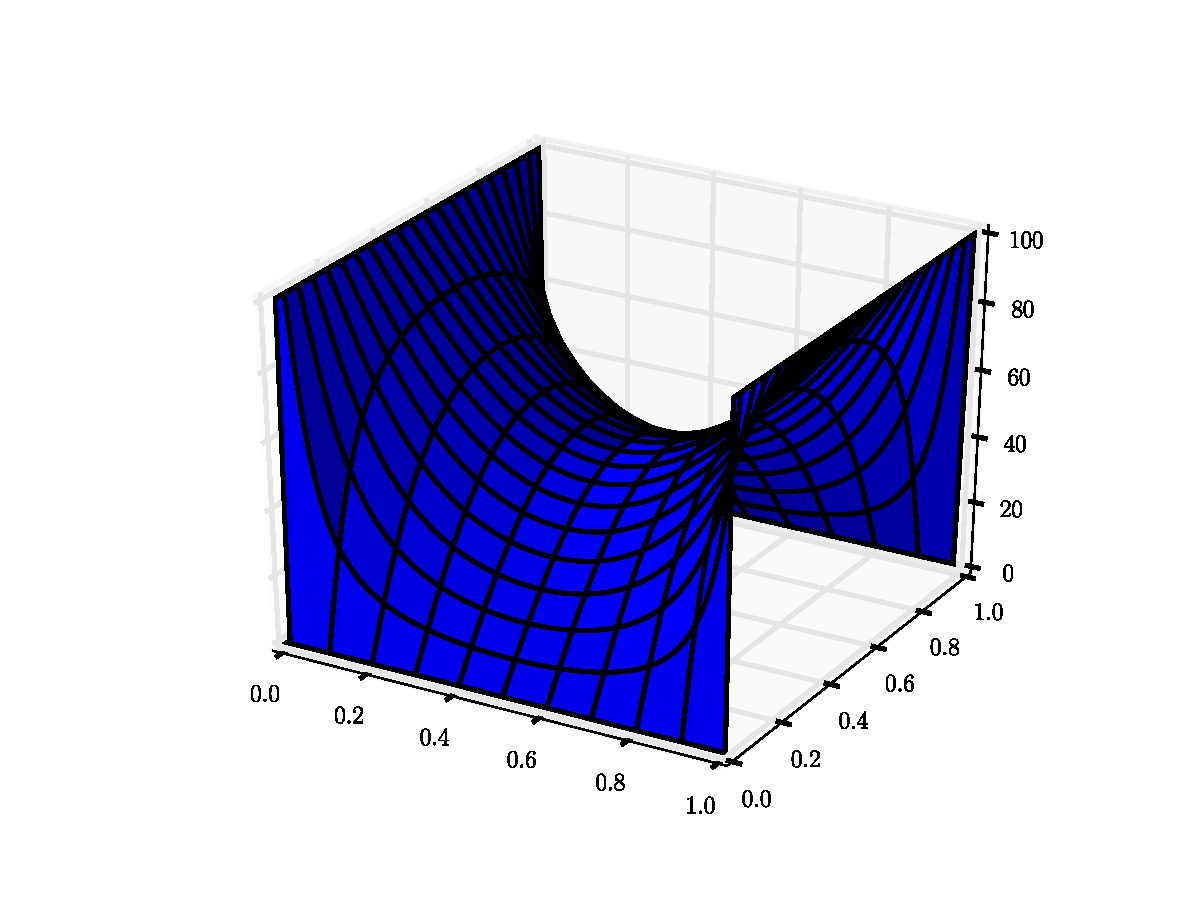
\includegraphics[width=.75\textwidth]{laplace.pdf}
\end{figure} 
\end{problem}


\begin{comment}
\section*{Saving Arrays} It is often useful to save an array as a file.
NumPy provides several easy methods for saving and loading array data.

\begin{table*}
\begin{tabular}{l|l}
\hline
\li{np.save(file, arr)} & Save an array to a binary file \\
\li{np.savez(file, *arrs)} & Save multiple arrays to a binary file \\
\li{np.savetxt(file, arr)} & Save an array to a text file \\
\hline
\end{tabular}
\end{table*}

\begin{table*}
\begin{tabular}{l|l}
\hline
\li{np.load(file)} & Load and return an array from a binary file \\
\li{np.loadtxt(file)} & Load and return an array from text file \\
\hline
\end{tabular}
\end{table*}

Let's practice saving an array to a file and loading it again.
Note that, when saving an array, NumPy automatically appends the extension \li{.npy} if it is not already present.
\begin{lstlisting}
a = np.arange(30)
np.save('test_arr', a)
new_a = np.load('test_arr.npy')
np.savez('test_multi', a=a, new_a=new_a)
arrs = np.load('test_multi.npz')
\end{lstlisting}
The variable \li{arrs} points to a dictionary object with the keys \li{a} and \li{new_a} which reference the arrays that have been saved.
The \li{.npz} file extension is the file type used to store multiple arrays.
\end{comment}

\begin{comment}
%%%%%%%%%%%%%%%%%%%%%%%%%%%%%%%%%%%%%%%%%%%%%%%%%%%%%%%%%%
\subsection*{Manipulating Arrays} 
Sometimes it is best to work on the entire array in single dimension. 
NumPy provides several ways to do this, each optimized for a different purpose.

The function \li{np.ravel()} returns a 1-D view of an array. It behave exactly like calling \li{reshape(-1)} on the array, but it executes faster.On the other hand, the array method \li{flatten()} returns a 1-D copy of the array.

Finally, the array method \li{flat} lets you iterate over the array as if it were 1-dimensional. Here is an example.
\begin{lstlisting}
>>> a = np.arange(4).reshape(2, 2)

# Iterate through the rows of a
>>> for i in a:
...     print i,
...     
[0 1] [2 3]

# Iterate through the entries of a
>>> for i in a.flat:
...     print i,
...
0 1 2 3
\end{lstlisting}
\end{comment}







%%%%%%%%%%%%%%%%%%%%%%%%%%%%%%%%%%%%%%%%%%%%%%%%%%%%%%%%%%%%%%%%%%%
%%%%%%%%%%%%%%%%%%%%%%%%%%%%%%%%%%%%%%%%%%%%%%%%%%%%%%%%%%%%%%%%%%%
%%%%%%%%%%%%%%%%%%%%%%%%%%%%%%%%%%%%%%%%%%%%%%%%%%%%%%%%%%%%%%%%%%%
%%%%%%%%%%%%%%%%%%%%%%%%%%%%%%%%%%%%%%%%%%%%%%%%%%%%%%%%%%%%%%%%%%%
%%%%%%%%%%%%%%%%%%%%%%%%%%%%%%%%%%%%%%%%%%%%%%%%%%%%%%%%%%%%%%%%%%%
\section*{NumPy and SciPy}
We now introduce some additional features of NumPy and SciPy.

\subsection*{Broadcasting Array Dimensions}
Many matrix operations make sense only when the two operands have the same shape. Two examples are addition and component-wise multiplication. Broadcasting is NumPy's way of extending such operations to accept some (not all) operands with different shapes. Broadcasting happens automatically whenever it is necessary. 

To understand broadcasting, let us look at an example. 
\begin{lstlisting}
>>> A = np.ones(3); A
array([ 1.,  1.,  1.])
>>> B = np.vstack([1, 2, 3]); B
array([[1],
       [2],
       [3]])
>>> A+B
array([[ 2.,  2.,  2.],
       [ 3.,  3.,  3.],
       [ 4.,  4.,  4.]])
\end{lstlisting}
We will now describe the algorithm used to obtain the result for \li{A+B} above. First, the shapes of \li{A} and \li{B} are lined up, starting at the far right, and 1's are prepended to the shorter tuple. So
\begin{lstlisting}
A 	(1-D array):     3
B	(2-D array): 3 x 1
\end{lstlisting}
becomes
\begin{lstlisting}
A 	(1-D array): 1 x 3
B	(2-D array): 3 x 1
\end{lstlisting}
For broadcasting to work, the dimensions must be compatible; that is, in a given axis, (1) they are equal, or (2) one of them is 1. Second, the arrays \li{A} and \li{B} are ``stretched'' one axis at a time until their dimensions are the same. In each axis, if the dimensions are different, the smaller array is copied along that axis (or ``stretched''), until it is the size of the larger array. Conceptually, we are creating new $3 \times 3$ arrays $A'$ and $B'$ where
\[
A' = \left[ \begin{array}{ccc}
1 & 1 & 1\\
1 & 1 & 1\\
1 & 1 & 1 \end{array} \right] \qquad \text{and} \qquad B' =  \left[ \begin{array}{ccc}
1 & 1 & 1\\
2 & 2 & 2\\
3 & 3 & 3\end{array} \right].
\]
Finally, NumPy returns the sum $A'+B'$.

We emphasize that the ``stretching'' in this example is only conceptual, and no new array $A'$ or $B'$ is created. However, 
you should still be careful when broadcasting large arrays because you can fill the 
RAM on your computer, which can sometimes freeze the system completely.
For a more detailed description of array broadcasting rules, see 
\url{http://docs.scipy.org/doc/numpy/user/basics.broadcasting.html}.

\begin{problem}
Create a $100\times100\times3$ array of integers taking values in the range 
[0, 256]. Such an array can represent an RGB image of $100\times100$ pixels, 
where each pixel is associated with an array of three integers indicating the 
amounts of red, green, and blue color present in that pixel, respectively.
Use array broadcasting to multiply the red and green values by $0.5$. 
(Such an operation would tone down the red and green colors and make the 
image appear more blue.) 
\end{problem}

\section*{Universal Functions}

A universal function, or \li{ufunc}, operates on an array elementwise. It outputs an array of the same shape and datatype as the input array. Using a universal function is usually much faster than iterating through the array yourself.

Many scalar functions from the Python standard library have a universal analog that operates on arrays. For example, \li{math.sin()} operates on scalars, and \li{numpy.sin()} operates on arrays. If you have a simple operation that you wan to perform elementwise on an array, you should see if SciPy has a universal function that will do it (it probably does). For a list of available \li{ufuncs}, see \url{http://docs.scipy.org/doc/numpy/reference/ufuncs.html#available-ufuncs}.

Most universal functions also allow you to specify an output array, which must have the same shape as the input array.
Doing so can reduce memory allocation. 

\begin{lstlisting}
>>> A = np.arange(3, dtype=float)

# Take exp(A) and store the result in A.
>>> np.exp(A, out=A) 
>>> A
array([ 1.        ,  2.71828183,  7.3890561 ])
\end{lstlisting}

\begin{comment}
Other useful examples are \li{max}, \li{min}, \li{absolute}, and \li{average}.
Each of these operations also allows you to specify whether you want to 
operate across a particular axis or over the entire array.
For example:

The above example returns a row of A which represents the maximum of all the 
rows of A. If we had set \li{axis=1}, it would have taken the maximum of all 
the columns. If, for purposes of broadcasting (discussed later) you need the 
output of one of these functions to have the same number of dimensions as the 
original array, you can also include the argument \li{keepdims=True}.

\end{comment}


Although universal functions also accept scalar inputs, they can be much slower than the corresponding standard library function. Thus, use standard library functions on scalars and universal functions on arrays.

\begin{comment}

\begin{lstlisting}
>>> timeit np.sin(.5)
1000000 loops, best of 3: 1.37 muµs per loop
>>> timeit np.math.sin(.5)
10000000 loops, best of 3: 144 ns per loop
\end{lstlisting}

We can see that performance increases when we know how to use a 
\texttt{ufunc}. However, they should only be used on arrays as they are 
not designed to handle single values efficiently.
\end{comment}

\section*{Linear Algebra}
Both NumPy and SciPy have a linear algebra library, but the SciPy library is larger. The SciPy linear algebra library is typically imported as follows.

\begin{lstlisting}
from scipy import linalg as la
\end{lstlisting}

\begin{comment}
To shorten the amount of typing, it can be aliased as 
\li{from scipy import linalg as la}.
\end{comment}

The linear algebra library contains several functions to construct special 
matrices, located in 
\li{linalg.special_matrices}. There are also functions that will invert matrices, find determinants and norms, solve linear systems and least squares problems, and find special matrix decompositions. You can read more about the linear algebra capabilities of SciPy in the 
documentation for the \li{linalg} module found at
(\url{http://docs.scipy.org/doc/scipy/reference/linalg.html}).

Finally, the \li{scipy.linalg} library has a \li{matrix} class that is very 
similar to a 2-D NumPy array. The matrix class can be convenient when doing matrix 
operations. However, in such situations we still recommend using NumPy arrrays, which have many of the same features and are also compatible with all other SciPy operations.

\begin{comment}
\begin{problem}
Block ciphers are ciphers that encode blocks of input symbols at a time 
instead of one symbol at a time. In the days before computers, the Hill 
cipher was the first cipher that allowed practical encoding of more than 
three symbols at a time. It was invented by Lester Hill in 1929.
The Hill cipher is considered a classical substitution cipher.
The entire cipher is based on linear algebra and uses a matrix key.
All substitution ciphers work with the 26 letters.
Thus, all our operations will be done mod 26 (modulo 26).
To do this, we introduce you to the \li{\%} operator in Python.
This new operator allows us to do modular arithmetic.
When applied to an array it takes the elementwise mod.

This problem has a number of parts.  You will write a function that 
accepts \emph{plaintext} and returns the encoded \emph{ciphertext}.
You will also write a decoder that will accept ciphertext and return 
plaintext.

The Encoder: \begin{enumerate}
\item We must first gather the plaintext to encode and a block size, $n$.
We must split this plaintext into blocks removing any spaces.  We need to 
convert each character to a number. We use the index of \li{string.lowercase} 
(found in the \li{string} module of the Python standard library).
We can easily build a lookup table that will let you easily find the index.
With a lookup table, we map each letter to its index.

\begin{lstlisting}
from string import lowercase
lut = {a:i for i, a in enumerate(lowercase)}
s = "this is a message"
s = "".join(s.split()) #remove all whitespace
map(lut.__getitem__, s) #return a list of indices
[19, 7, 8, 18, 8, 18, 0, 12, 4, 18, 18, 0, 6, 4]
\end{lstlisting}

Another way is to use \li{lowercase.index()} in a loop to find the index 
each time.
% \begin{lstlisting}
% >>> indices = []
% >>> for letter in s:
%         indices.append(lowercase.index(letter))
% \end{lstlisting}
We need to split the list of indices into $n$-length arrays and store them 
in a list. If the input is not a multiple of $n$, you will need to pad the 
input until it is a multiple of $n$. Pick any character to pad the input 
(typically it is a rarely used letter). The \li{itertools} module is useful 
for this.  One of the common recipes for doing this task is available in 
the \li{itertools} documentation.

\begin{lstlisting}
def grouper(iterable, n, fillvalue=None):
    "Collect data into fixed-length chunks or blocks"
    # grouper('ABCDEFG', 3, 'x') --> ABC DEF Gxx
    args = [iter(iterable)] * n
    return itertools.izip_longest(fillvalue=fillvalue, *args)
\end{lstlisting}

It will be useful to wrap all of this step in a separate function as we will 
need to do the same thing when decoding (except for removing whitespace).

\item Find a suitable cipher key.  The keys of a Hill cipher are square 
matrices.  Let $K$, be our key. $K$ must be invertible mod 26.
Remember from linear algebra, that the determinant of square matrix will 
tell you if that matrix is invertible. To find a matrix that is invertible 
mod 26, we need to find a matrix with a determinant that is relatively prime 
to 26 (they share no common factors). The Euclidean algorithm can be used to 
determine if two numbers are co-prime (i.e. $\gcd(d, 26) = 1$). Write a 
function that generate random integer matrices using NumPy, checking the 
determinant, and returns a suitable key, $K$.

\item Write a function that will accept a message and a key matrix.
The message should already be broken into $n$ length blocks (you can do this 
inside the encode function if needed) and the matrix should be $n \times n$.
A Hill cipher is the dot product of the block with the key.  Return a 
ciphertext that is letters (the numbers correspond the indices in 
\li{string.lower}).

\item Write a function that will compute $K^{-1} \pmod{26}$.  This will 
necessarily be an integer inverse.
Use \li{linalg.inv} to find the inverse of $K$.
Then \[K^{-1} = \det(K)K^{-1}\det(K)^{-1}  \pmod{26}\] where $\det(K)^{-1}$ 
is the inverse of the determinant mod 26.
You will need to round the determinant to the nearest integer before doing 
these steps.  You will also need to round the results of each of your 
multiplications.
You can check that you have the integer inverse by checking $KK^{-1} = I$.

\item Write a function that will decode a message given a ciphertext and the 
key. You will need to invert the key before decoding.  Break the message into 
blocks of size $n$ and calculate the dot product of each block with the 
inverted key. Return a plaintext that is letters (the numbers, again, 
correspond to indices in \li{string.lower}).
\end{enumerate}

Experiment with your Hill cipher.  If you are in a classroom setting, try 
sending encoded messages to friends (they will need the key you used to 
encode).
\end{problem}
\end{comment}

\section*{Polynomials}
The \li{np.poly1d} object represents polynomials in NumPy. The constructor is called with the coefficients of the desired polynomial. 

\begin{lstlisting}
>>> a = np.poly1d([3, 5, 1, 2, 0, 1])
>>> print a
   5     4     3     2
3 x + 5 x + 1 x + 2 x + 1
\end{lstlisting}

The object \li{a} represents the polynomial $3x^5+5x^4+x^3+2x^2+1$.
NumPy provides many functions to operate on \li{poly1d} objects (see \url{http://docs.scipy.org/doc/numpy/reference/routines.polynomials.polynomial.html}).

\begin{comment}
\begin{table}
\centering
\begin{tabular}{l|l}
Function & Description \\
\hline
\li{np.polyadd} & Add two polynomial arrays \\
\li{np.polyder} & Find the derivative of a polynomial array \\
\li{np.polydiv} & Divide two polynomial arrays \\
\li{np.polyfit} & Find a least squares polynomial fit \\
\li{np.polyint} & Find the integral of a polynomial array \\
\li{np.polymul} & Multiply two polynomial arrays \\
\li{np.polysub} & Subtract two polynomial arrays \\
\li{np.polyval} & Evaluate a polynomial at specific points
\end{tabular} \caption{A few methods of NumPy polynomial arrays.}
\label{poly1dmethods}\end{table}
\end{comment}

Here is an example using the \li{poly1d} class. Recall that
\[
e^x = \sum_{n=0}^{\infty} \frac{x^n}{n!}.
\]
The following function evaluates the $n^{th}$ partial sum of this series at the value $a$.

\lstinputlisting[style=fromfile]{exp.py}
\begin{comment}
\begin{lstlisting}
from scipy.misc import factorial
n = 18 # number of terms
p = 1. / factorial(np.arange(18, -1, -1)) # compute coefficients
X = np.random.rand(10000) # where to evaluate the series
P = np.poly1d(p) # make polynomial object
P(X)
\end{lstlisting}
\end{comment}
The last two lines can be condensed by using

\begin{lstlisting}
np.polyval(p, a)
\end{lstlisting}

\begin{problem}
\begin{enumerate}[a)]
\item Use the NumPy's polynomial objects to approximate the following series.
\[
\arcsin x = \sum_{n=0}^{\infty} \frac{\left(2 n\right) ! x^{2 n + 1}}{\left(2 n + 1\right)\left(n!\right)^2 4^n}
\]
Use your approximation to find a close approximation of $\pi$. Hint: think of the powers of $x$ that
are not included in the series as having zero coefficients.

\item The lambert W function is the inverse of $x e^x$.
It's taylor series is
\[
W(x) = \sum_{n=1}^{\infty} \frac{\left(-n\right)^{n-1} x^n}{n!}
\]
This series has a radius of convergence of $\frac{1}{e}$.
Use the series to find a number $x$ such that $x e^x = \frac{1}{4}$.
Verify that your computation is correct.

(Note: Be careful with your indices; check to see where each taylor series begins!)
\end{enumerate}
\end{problem}

\begin{comment}
\section*{Useful Functions}
The following table contains a list of useful NumPy functions. 
For more information please refer to the NumPy documentation.
\begin{table}
\centering
\begin{tabular}{l|l}
Function & Description \\
\hline
\li{np.intersect1d} & Return the intersection of two flattened arrays. \\
\li{np.union} & Return the union of two flattened arrays. \\
\li{np.diff} & Calculates a discrete difference of order $n$. \\
\li{np.absolute} & Return the elementwise absolute value of an array. \\
\li{np.pad} & \\
\li{np.nonzero} & \\
\li{np.count_nonzero} & \\
\li{np.select} & \\
\li{np.nan} & Represent IEEE NAN (not-a-number). \\
\li{np.inf} & Represent IEEE INF (infinity). \\
\li{np.who} & Print information about defined NumPy arrays in a variable scope. \\
\li{np.unique} & Return a sorted array of unique elements of an array. \\
\end{tabular} 
\end{table}
\end{comment}

\section*{Specifications}
We suggest that you submit your \li{solutions.py} file using the following format.
\begin{lstlisting}
import math
import timeit
import string
import itertools
import numpy as np
from fractions import gcd
from numpy.random import randn
from scipy import linalg as la
from scipy.misc import factorial
from matplotlib import pyplot as plt
from mpl_toolkits.mplot3d import Axes3D

# Problem 1

def arr_mult(A,B):
    new = []
    for i in range(len(A)):
        newrow = []
        for k in range(len(B[0])):
            tot = 0
            for j in range(len(B)):
                tot += A[i][j] * B[j][k]
            newrow.append(tot)
        new.append(newrow)
    return new
    
def timefunction(f, *args, **kwargs):
	pfunc = lambda: f(*args, **kwargs)
	print min(timeit.repeat(pfunc, number = 1, repeat = 1))

def problem1():
	print "LIST: k = 100: <time>"
	print "LIST: k = 200: <time>"
	print "LIST: k = 300: <time>"
	print "ARRAY: k = 100: <time>"
	print "ARRAY: k = 200: <time>"
	print "ARRAY: k = 300: <time>"
	
'''
Response to question
'''

# Problem 2

def problem2():
    print "A.reshape(A.size) had a best time of <time>"
    print "A.flatten() had a best time of <time>"
    print "A.reshape((1, A.size)) had a best time of <time>"
    
'''
Response to question
'''

# Problem 3

def laplace(U, tol):
	pass
        
n = 100
tol = .0001	
U = np.ones((n, n ))
U [:,0] = 100 # set north boundary condition
U [:,-1] = 100 # set south boundary condition
U [0] = 0 # set west boundary condition
U [-1] = 0 # set east boundary condition
# U has been changed in place.
laplace(U, tol) 
x = np.linspace (0, 1, n)
y = np.linspace (0, 1, n)
X, Y = np.meshgrid (x, y)
fig = plt.figure()
ax = fig.gca( projection = '3d')
ax.plot_surface (X, Y, U, rstride=5)
plt.show()

# Problem 4

def problem4(n):
	return var
	
'''
Response to question
'''

# Problem 5

# [red, green, blue]
def problem 5():
	pass

# Problem 6

def arcsin_approx():
	return sol

def W_approx():
	return sol

\end{lstlisting}

